\subsection{Rotationskörper \texorpdfstring{\hfill S.75}{S.75}}
Alle Funktionen müssen strikt monoton sein. 
\subsubsection{Rotation um x-Achse}
    \begin{minipage}{0.5\linewidth}
        \begin{align*}
            V_x &= \pi \int_a^b (f(x))^2 dx \\
            V_x &= \pi \left\lvert \int_{t1}^{t2} y^2 \dot{x} dt \right\lvert   
        \end{align*}
    \end{minipage}
\begin{minipage}{0.49\linewidth}
    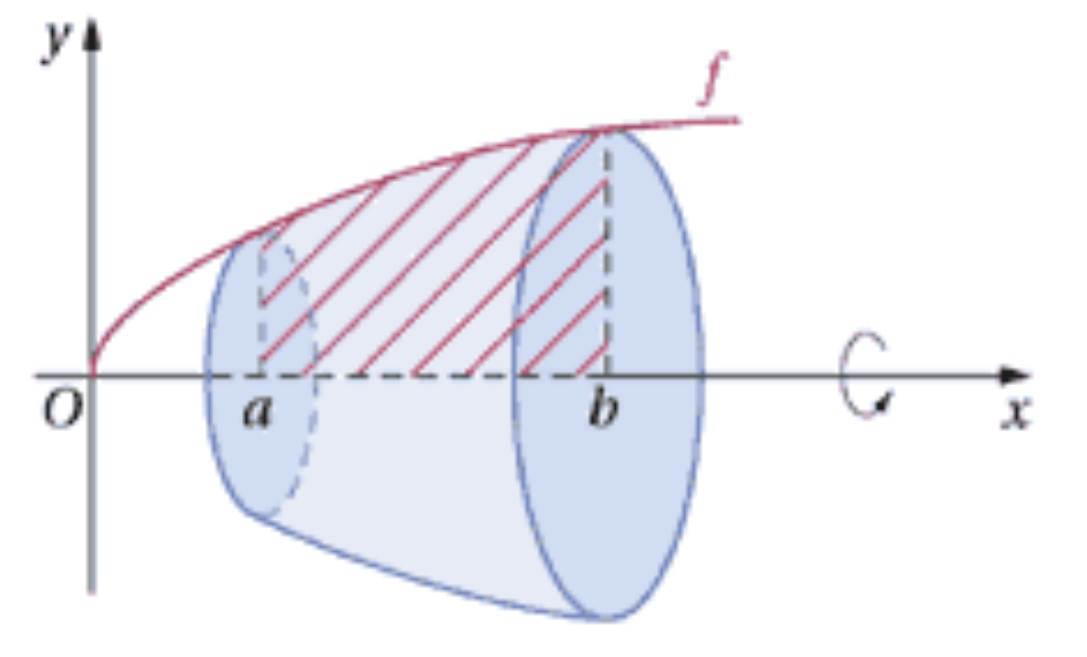
\includegraphics[width=\linewidth]{src/Mehrdimensionale-Funktionen_Integralrechnung/x_Achsen_Rotation.jpg}
\end{minipage}

\subsubsection{Rotation um y-Achse "disk integration"}
    \begin{minipage}{0.5\linewidth}
        \begin{align*}
             V_y &= \pi \int_a^b x^2 \cdot \left\lvert f'(x) \right\lvert dx \\
             V_y &= \pi \left\lvert \int_{t1}^{t2} x^2 \dot{y} dt  \right\lvert 
        \end{align*}
    \end{minipage}
    \begin{minipage}{0.49\linewidth}
         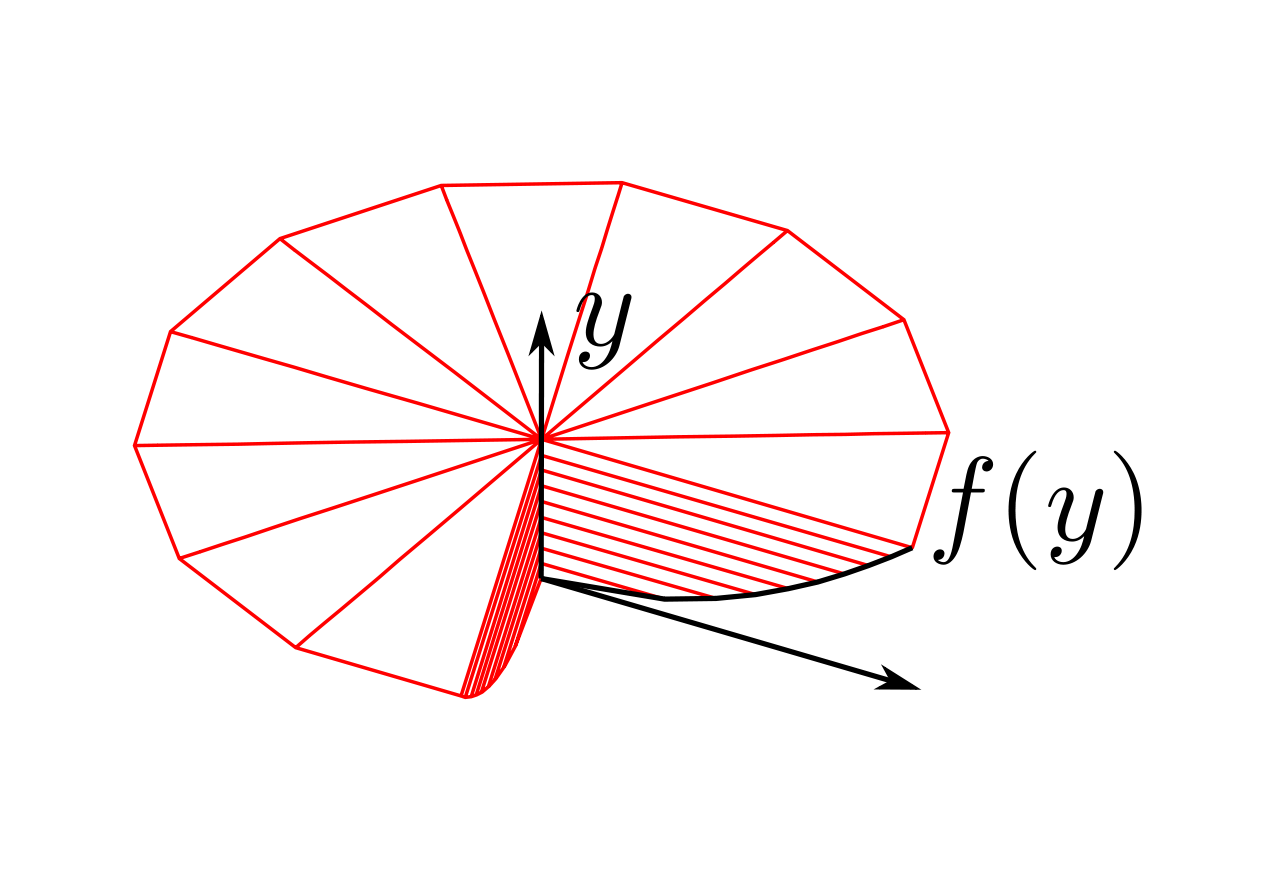
\includegraphics[width=\linewidth]{src/Mehrdimensionale-Funktionen_Integralrechnung/disk_integration.png}
    \end{minipage}

\subsubsection{Rotation um y-Achse "shell integration"}
    \begin{minipage}{0.5\linewidth}
        $$ V_y = 2\pi \int_a^b xf(x)dx $$
    \end{minipage}
    \begin{minipage}{0.49\linewidth}
         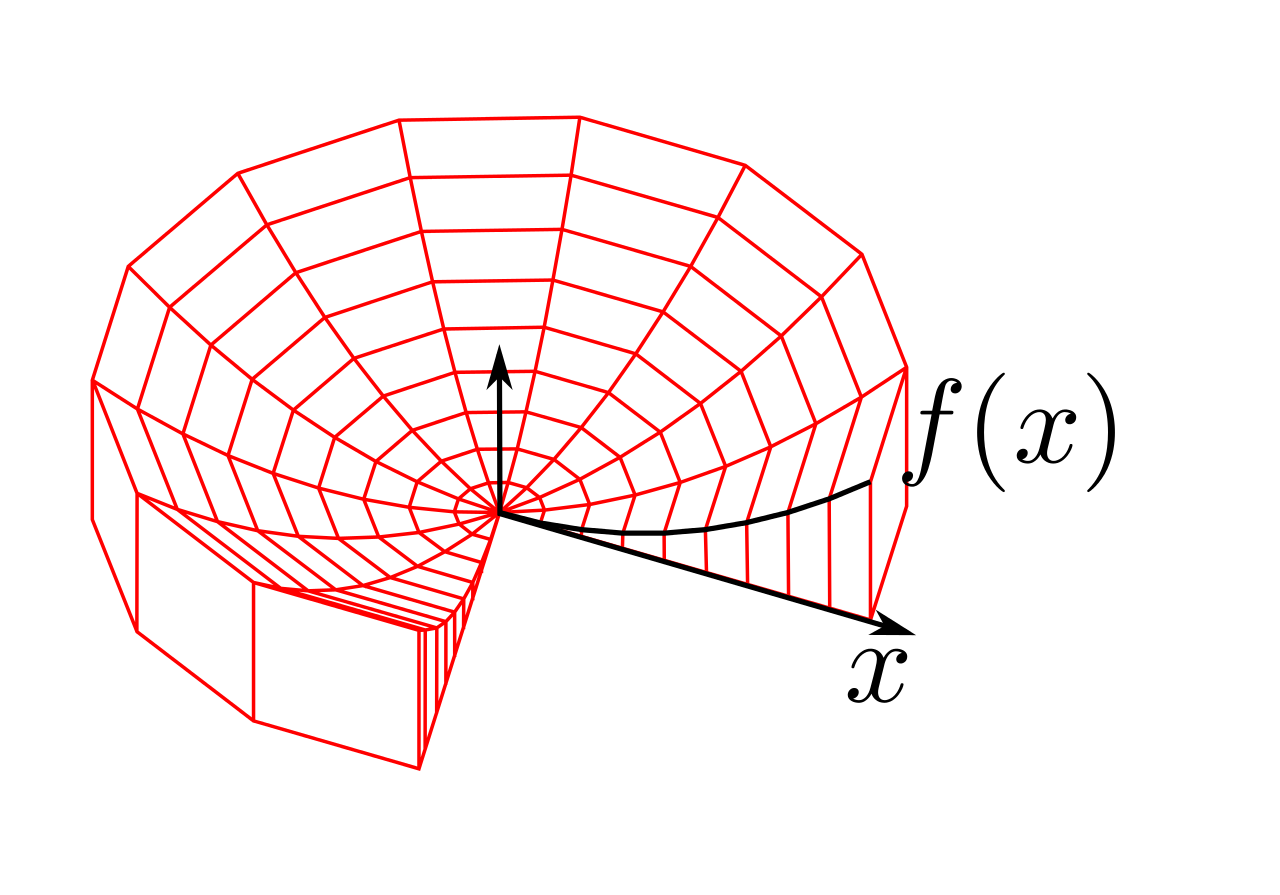
\includegraphics[width=\linewidth]{src/Mehrdimensionale-Funktionen_Integralrechnung/shell_integration.png}
    \end{minipage}


